\section{Findings}

The included studies cluster into four recurring architectural patterns. Table~\ref{tab:concept-matrix} summarizes these patterns by linking their dominant orchestration mechanisms to the engineering constraints they address and the primary studies assigned to each category. This concept matrix provides the organizing structure for the research-question-based analysis that follows.

\begin{table}[!htbp]
\centering
\caption{SLM--LLM architectural concept matrix.}
\label{tab:concept-matrix}
\footnotesize
\setlength{\tabcolsep}{3pt}
\renewcommand{\arraystretch}{1.08}
\begin{tabularx}{\linewidth}{
  @{}
  >{\raggedright\arraybackslash}p{0.16\linewidth}
  >{\raggedright\arraybackslash}p{0.25\linewidth}
  >{\raggedright\arraybackslash}p{0.22\linewidth}
  >{\raggedright\arraybackslash}X
  @{}
}
\toprule
\textbf{Architectural Pattern} &
\textbf{Orchestration Mechanism} &
\textbf{Key Engineering Constraints Addressed} &
\textbf{Primary Studies} \\
\midrule
\textbf{Hybrid Architectures} &
Token-level routing, draft-verification, uncertainty-aware skipping, and edge--cloud distribution. &
API cost, edge--cloud bandwidth, and latency thresholds. &
\mbox{S2}, \mbox{S13}, \mbox{S27}, \mbox{S32}, \mbox{S33}, \mbox{S45}, \mbox{S46}, \mbox{S48}, \mbox{S49}, \mbox{S53}. \\

\textbf{Multi-Agent Systems} &
Role specialization, iterative verification, adversarial debate, and feedback loops. &
Reasoning depth, logical accuracy, and complex task decomposition. &
\mbox{S1}, \mbox{S6}, \mbox{S7}, \mbox{S11}, \mbox{S15}, \mbox{S16}, \mbox{S20}, \mbox{S29}, \mbox{S37}, \mbox{S43}, \mbox{S51}, \mbox{S52}, \mbox{S54}. \\

\textbf{Retrieval-Centered (RAG)} &
Adaptive retrieval planning, context expansion, fact-grounding, and action-space constraint. &
Hallucination reduction, data privacy, and strict domain accuracy. &
\mbox{S4}, \mbox{S10}, \mbox{S21}, \mbox{S30}, \mbox{S31}, \mbox{S44}. \\

\textbf{Ensembles and Heterogeneous Fusion} &
Tabular transformation, cross-modal late fusion, and prompt-guided multimodal sampling. &
Hardware limits on central processing units (CPUs) and edge devices, and non-text modality processing. &
\mbox{S3}, \mbox{S5}, \mbox{S8}, \mbox{S9}, \mbox{S12}, \mbox{S14}, \mbox{S17}, \mbox{S18}, \mbox{S19}, \mbox{S22}, \mbox{S23}, \mbox{S24}, \mbox{S25}, \mbox{S26}, \mbox{S28}, \mbox{S34}, \mbox{S35}, \mbox{S36}, \mbox{S38}, \mbox{S39}, \mbox{S40}, \mbox{S41}, \mbox{S42}, \mbox{S47}, \mbox{S50}. \\
\bottomrule
\end{tabularx}
\end{table}

\subsection{Systematic Map of the Literature}

Before addressing the specific research questions, we present a systematic map of the 54 included primary studies to provide visual context for the field's current trajectory. As illustrated in Figure~\ref{fig:publication-years}, the distribution of publication years reveals a sharp acceleration in SLM--LLM collaborative research. While early foundational work on model adaptation appeared in 2023, the vast majority of the corpus (39 studies, 72.2\%) was published in 2025, underscoring that architectural orchestration---rather than standalone model scaling---is a rapidly maturing engineering priority.

\begin{figure}[!htbp]
\centering
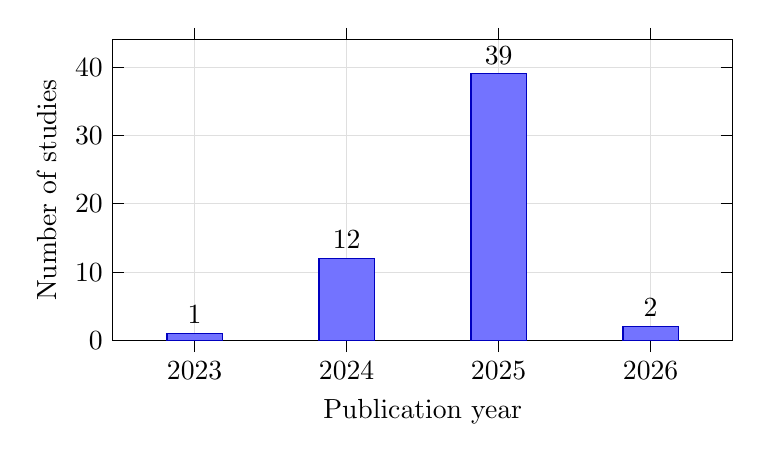
\begin{tikzpicture}
\begin{axis}[
    ybar,
    width=0.78\linewidth,
    height=5.4cm,
    ymin=0,
    ymax=44,
    ytick={0,10,20,30,40},
    ylabel={Number of studies},
    symbolic x coords={2023,2024,2025,2026},
    xtick=data,
    xlabel={Publication year},
    bar width=20pt,
    nodes near coords,
    nodes near coords align={vertical},
    enlarge x limits=0.18,
    axis line style={black},
    tick style={black},
    grid=major,
    grid style={draw=gray!25},
]
\addplot[fill=blue!55, draw=blue!75!black] coordinates {
    (2023,1)
    (2024,12)
    (2025,39)
    (2026,2)
};
\end{axis}
\end{tikzpicture}
\caption{Publication-year distribution of the 54 included primary studies.}
\label{fig:publication-years}
\end{figure}

Figure~\ref{fig:domain-distribution} visualizes the distribution of applied domains across the literature. The studies are heavily concentrated in areas requiring strict logical reasoning, such as software engineering, mathematics, and related logical-reasoning tasks (11 studies, 20.4\%), and fields governed by severe privacy and latency constraints, namely healthcare and medicine (10 studies, 18.5\%) and telecommunications, edge, and networking (10 studies, 18.5\%). This distribution confirms that hybrid and multi-agent systems are primarily engineered to solve domain-specific operational bottlenecks rather than general-purpose generative tasks.

\begin{figure}[!htbp]
\centering
\begin{tikzpicture}
\pie[
    sum=54,
    radius=2.45,
    text=legend,
    before number={},
    after number={\ studies},
    color={
        blue!65,
        red!60,
        teal!65,
        orange!75,
        violet!60,
        brown!65,
        gray!65
    }
]{
    11/{Software, mathematics, and logical reasoning},
    10/{Healthcare and medicine},
    10/{Telecommunications, edge, and networking},
    10/{General NLP, sentiment, and benchmarking},
    7/{Specialized scientific and spatial},
    3/{Cybersecurity and threat intelligence},
    3/{Energy and resource optimization}
}
\end{tikzpicture}
\caption{Primary applied-domain distribution of the 54 included studies. Categories reflect each study's principal evaluation domain; methodologically overlapping studies are assigned to one primary category for this aggregate view.}
\label{fig:domain-distribution}
\end{figure}

\subsection{RQ1: Comparative Performance of Hybrid and Multi-Agent Systems}

The review shows that both hybrid and multi-agent architectures can outperform standalone small-model baselines, but their advantages emerge through different forms of coordination rather than parameter scaling alone. Hybrid systems achieve their strongest gains when computation is selectively distributed between local small models and stronger remote models. Token-level edge--cloud collaboration improves small-model performance without requiring full-query escalation: draft-verification, low-confidence routing, and uncertainty-aware skipping allow small models to approach LLM-level quality while invoking the larger model selectively (S13, S48, S49). At the sub-task level, structured task decomposition and cloud--edge allocation also maintain reasoning accuracy comparable to the best baselines (S14). In domain-specific settings, hybrid orchestration can outperform larger general-purpose models: a fine-tuned Phi-2 (2.7B) combined with retrieval, reranking, hybrid search, and long-context support achieves 84.20\% accuracy, exceeding GPT-4o mini (82.05\%) and GPT-4o (80.80\%) on telecommunications question answering (QA) (S17).

Multi-agent systems, by contrast, show their comparative strength when performance depends on role specialization, critique, verification, and distributed reasoning. A three-agent Phi-3-based architecture performs on par with human experts in conceptual genomics tasks, although its gains weaken on more complex code-generation workflows, indicating that multi-agent benefits remain task-sensitive (S52). In reasoning-intensive question answering, a Proponent--Opponent--Arbitrator structure built on compact models such as Qwen2.5 0.5B and DeepSeek-R1 1.5B surpasses both single-agent reasoning and vanilla LLM baselines (S43). Likewise, assistant--checker collaboration supported by memory and feedback loops enables small-model multi-agent systems to approach or exceed larger baselines across database, knowledge-graph, and code-correction tasks (S29). Overall, the findings indicate that hybrid systems are most effective when the main challenge is balancing accuracy with latency and cost through adaptive routing, whereas multi-agent systems are most effective when the task benefits from explicit decomposition of reasoning roles and iterative verification. Thus, the comparative performance advantage of both architecture families is driven primarily by orchestration strategy, not by model size alone.
\subsection{RQ2: Efficiency, Cost, Latency, and Energy Trade-offs}

Efficiency motivates many hybrid and multi-agent systems, but the impact on cost, latency, and energy depends heavily on orchestration. Hybridization is not a universal efficiency solution; it often shifts bottlenecks rather than eliminating them.

Regarding inference cost and token consumption, architectures employing selective escalation or task decomposition drastically reduce reliance on massive standalone LLMs. S49 achieves an over 80\% cost reduction compared to full LLM inference by routing fewer than 7\% of generated tokens to the cloud. Similarly, S13 uses a token-level draft-verification method to match the quality of a 70B parameter LLM while consuming only 25.8\% to 31.2\% of standard cloud inference costs. Query-level decomposition yields similar savings: S14 cuts average API costs by 83.57\% via parallel reasoning. Computational savings are also heavily emphasized through token reduction. S40 achieves a 95\% reduction in LLM token transmissions via federated uncertainty-aware routing, and S15 eliminates redundant multi-round communications through an SLM-generated directed acyclic graph, reducing token consumption by 35\% to 70\%. In dialogue state tracking, S16 highlights that a retrieval-based router reduces overall floating-point operations (FLOPs) by approximately 62\%.

Conversely, the impact on latency is highly polarized. In optimal scenarios, relying on lightweight models accelerates throughput: a fine-tuned SLM in a hybrid classification pipeline (S10) operates at 7.41 ms on a graphics processing unit (GPU), and uncertainty-aware skipping in an edge--cloud setup provides 2.54$\times$ faster token throughput (S48). However, orchestration mechanisms frequently introduce new bottlenecks. Planners and retrievers add temporal overhead, as shown by the adaptive retrieval planner in S11 (1.42 seconds versus 0.95 seconds for naive retrieval) and by cross-encoder reranking in S17. Multi-agent collaboration also multiplies inference cycles: S43 reports a 1.8$\times$ inference-time overhead for adversarial debate, while complex agentic workflows can push average response latency to 107 seconds (S31). Processing time is further affected by hardware and modality constraints, including constrained local hardware, dual-path video sampling, CPU-only ensembles, and key-value cache recomputation at the edge (S20, S23, S50, S5).

Energy consumption remains the least documented metric in the reviewed studies, and most reported efficiency gains are resource proxies rather than direct energy measurements. The clearest energy-centered evidence comes from S4, which argues for energy-per-token as a more informative metric and shows that forcing a small model to execute complex reasoning workflows, such as Chain-of-Thought, can substantially increase its per-query energy use. In some settings, a larger model prompted more directly is therefore more energy-efficient than a smaller model that generates a long reasoning trace. By contrast, S29 reports a 26.4\% reduction in computational redundancy through dual-scale memory, which may indicate lower resource demand but does not by itself constitute a direct energy benchmark. Taken together, the review suggests that energy efficiency depends on orchestration and generation length as much as on model size, and that stronger claims require standardized, hardware-specific measurement protocols.

\subsection{RQ3: Orchestration and Routing Mechanisms}
The studies contain a broad set of orchestration mechanisms, but they can be organized into a small number of recurring families. Across the included studies, performance differences are explained less by absolute model size than by how effectively the system retrieves evidence, routes uncertainty, and divides labor across components.

Token-level orchestration is most visible in verification-oriented hybrid systems. S13 uses the SLM as a drafter and the LLM as a verifier on difficult tokens. S48 extends this pattern with uncertainty-aware skipping so that likely acceptable SLM tokens can bypass the remote model. S49 reaches a related design point by routing only low-confidence tokens for external inference. Taken together, these studies show that token-level collaboration provides fine-grained control over answer quality, but it can also introduce communication and synchronization overhead when escalation rates increase.

Query-level routing appears when the system selects a processing path for the full input rather than for individual tokens. S16 exemplifies retrieval-based expert routing at the dialogue level, while S10 shows that instance-level model selection can also be effective in customer-review analysis. These designs are most useful when ``easy'' and ``hard'' cases can be separated in a semantically meaningful way before full generation begins.

RAG is a major control mechanism across the included studies even when the architecture is classified as hybrid rather than purely RAG. S17, S11, S39, and S47 use retrieval not only to expand context but also to constrain the action space of a smaller model. In these studies, retrieval acts as a coordination layer that narrows ambiguity, grounds the answer in domain evidence, and reduces reliance on raw model scale alone.

Task decomposition is increasingly important in the recent literature. S14 uses a task decomposer, dependency graph, and plug-and-play adapter to allocate subtasks between local and remote models. S53 uses a feedback-integrated workflow that gathers structured feedback from multiple perspectives before revising the prompt of the smaller model. Related role-based decomposition also appears in S23, S29, and S52. Across these studies, the common idea is that small models remain viable when the workflow can be partitioned into specialist stages rather than handled as a single undifferentiated generation step.

Orchestration frequently extends beyond unimodal text processing to integrate diverse data modalities and specialized neural architectures. Several frameworks are designed to fuse language models with non-text representations and structured data. For example, S20 combines coarse-grained and fine-grained visual semantics through prompt-guided video sampling, while S8 fuses language-model embeddings with graph-convolutional features for molecular-property prediction. This heterogeneous routing is particularly prevalent in applied domains such as medicine; S19 orchestrates convolutional networks (ConvNeXt) for anatomical localization alongside a self-reflective LLM agent, and S34 employs a late-fusion approach to combine structured gradient boosting models based on electronic health record (EHR) tabular data with unstructured clinical text analysis. In these settings, orchestration operates as a structured fusion mechanism, ensuring that visual, spatial, or mathematical data is processed by the optimal specialized architecture before language generation occurs.

\subsection{RQ4: Domain Suitability and Application-Specific Constraints}
The choice between hybrid and multi-agent systems is rarely domain-agnostic. Privacy mandates, latency budgets, and verification demands largely determine the orchestration method. Across the 54 primary studies, distinct architectural preferences emerge across four core applied domains.

In fields with strict privacy constraints or high-stakes accuracy requirements, hybridization is driven by the need to keep data local while grounding the SLM in verifiable facts. Local SLMs fine-tuned on clinical corpora and augmented by RAG are therefore well suited to medical reporting and clinical classification tasks (S19, S30), while few-shot open-source models can be competitive for structured radiology labeling (S12). Related healthcare studies also show that local ensembles, tabular transformations, and distillation can support diagnostic or summarization workflows without relying on a fully remote LLM (S28, S33, S41). In scientific settings, structurally augmented SLMs can be effective when language representations are fused with domain-specific models, as in molecular property prediction with graph-convolutional features (S8).

Tasks requiring rigid syntax, iterative refinement, and logical debugging benefit from multi-agent or feedback-driven SLMs rather than zero-shot massive LLMs. Pedagogy, assessment, code correction, and database tasks favor workflows in which small models receive structure, memory, or explicit feedback (S6, S29, S32). In software and bioinformatics settings, role-specific agents can mimic developer-reviewer workflows and generate or revise code offline, although broad static analysis still favors larger models when the task requires open-ended type inference (S24, S2, S52, S53).

Telecommunications architectures prioritize latency budgets, bandwidth allocation, and domain-specific vernacular, making hybrid edge--cloud systems and retrieval-grounded SLMs the dominant pattern. Telecom QA benefits from fine-tuning, retrieval, reranking, and long-context support because these mechanisms ground smaller generators in technical standards and network terminology (S17, S47). Beyond QA, latency optimization and bandwidth reduction drive hybridization through lightweight prediction, uncertainty-aware skipping, and sub-task decomposition (S37, S48, S14).

In edge, cyber-physical, and multimodal settings, orchestration is governed by hardware limits and input modality. Mission-critical aerospace and geospatial workflows rely on local or distributed agents to process operational data under deployment constraints (S23, S45). Industrial video monitoring and cross-modal sensing benefit from heterogeneous pipelines in which local models handle coarse or sensor-side processing while larger multimodal models are invoked only for complex cases (S20, S1). Overall, these domains show that collaborative SLM--LLM systems are strongest when the workflow can be partitioned according to privacy, latency, modality, or verification needs.

\subsection{Cross-RQ Synthesis}
Viewed together, the four research questions suggest a consistent systems principle: hybrid language-model design works best when the large model is treated as a selectively invoked capability rather than the default engine for every token, query, or subtask.

Strong results are associated with explicit control layers such as routers, planners, retrievers, or fusion modules. Future progress is therefore unlikely to come only from making SLMs slightly larger or LLMs slightly cheaper; it will also depend on better confidence estimation, task decomposition, retrieval selection, and cross-model scheduling.

Methodologically, because accuracy dominates reporting, many studies overstate practical efficiency. The review includes cases where orchestration clearly reduces cost or latency, but also cases where coordination merely shifts the bottleneck. A mature evaluation protocol should therefore report resource metrics as first-class outcomes. Application-wise, the strongest SLM-centered deployments are domain-adapted systems in which the small model is grounded, specialized, or protected by escalation logic. This is why telecom, structured reasoning, radiology labeling, optimisation formulation, and industrial monitoring are prominent in the positive findings.

\subsection{Implications for Practitioners}
For software engineers and system architects, the main design trade-offs are operational rather than purely model-centric. In practice, latency, cost, privacy, and hardware constraints often dominate deployment decisions. Four practical design patterns emerge from the reviewed studies. When strict data privacy is the main constraint, local SLM + RAG architectures are most suitable for healthcare, telecom, and defense settings (S17, S23, S19, S30), but their performance depends heavily on retriever quality. When high throughput is required, hybrid edge--cloud architectures are appropriate for Internet of Things (IoT) and network traffic scenarios (S37, S40, S48, S49), reducing API costs while requiring careful threshold tuning. For logical reasoning tasks such as code and mathematics, multi-agent SLM designs can improve accuracy (S29, S15, S43, S52), but they introduce significant latency overhead. For multimodal data, heterogeneous fusion is better suited to medical imaging and robotics (S8, S20, S19, S1), although the slowest model in the pipeline often becomes the bottleneck. Three practitioner-facing principles follow: (1) \textbf{Design for routing}: orchestration, not model size, drives performance; (2) \textbf{Balance latency-cost trade-offs}: real-time tasks favor token skipping, while batch tasks tolerate multi-agent loops; and (3) \textbf{Treat RAG as control}: retrieval constrains the SLM action space and grounds outputs in verifiable facts.
